% !TEX root = ../main.tex
\newpage
\chapter{Реалізація програмної взаємодії з БД}
\section{Посібник користувача}
Попередньо на ПК має бути встановлено сервер MySQL 8.0 та інтерпретатор мови програмування Python 3.9.
Після запуску SQL-сервера перед першим запуском інформаційної системи необхідно
запустити файл setup.py (додаток 2, ст. \pageref{setup}), який виконає створення 
схеми БД на сервері, створить усі необхідні таблиці, створить усі необхідні для запитів процедури
та завантажить тестові дані до таблиць:
\begin{lstlisting}[style=code]
PS C:\Users\Yalikesi\...\campus> python setup.py
enter connection parameters:
        host (leave empty for default localhost):
        port (leave empty for default 3307):
        user (leave empty for default root):
        password for root:
creating schema and tables...
        done in 1.109 sec
inserting data...
        done in 28.481 sec
creating stored procedures...
        done in 0.227 sec
database is ready!
\end{lstlisting}
Після цього параметри підключення до БД буде збережено і можна буде запускати веб-інтерфейс за
допомогою файлу main.py: буде виведено рядок \inlinecode{Running on http://127.0.0.1:5000/ (Press CTRL+C to quit)},
який означатиме, що веб-інтерфейс доступний за адресою 127.0.0.1:5000. Його можна відкрити за допомогою
будь-якого сучасного браузера. Під час тестування коректність його роботи перевірялася в Google Chrome 90.
У веб інтерфейсі є можливість перегляду окремих таблиць БД та виконання передбачених запитів.
На всіх сторінках, де виводяться таблиці, є можливість сортування за кожним стовпцем та пошуку по виведеній таблиці.
\begin{figure}[H]
    \centering
    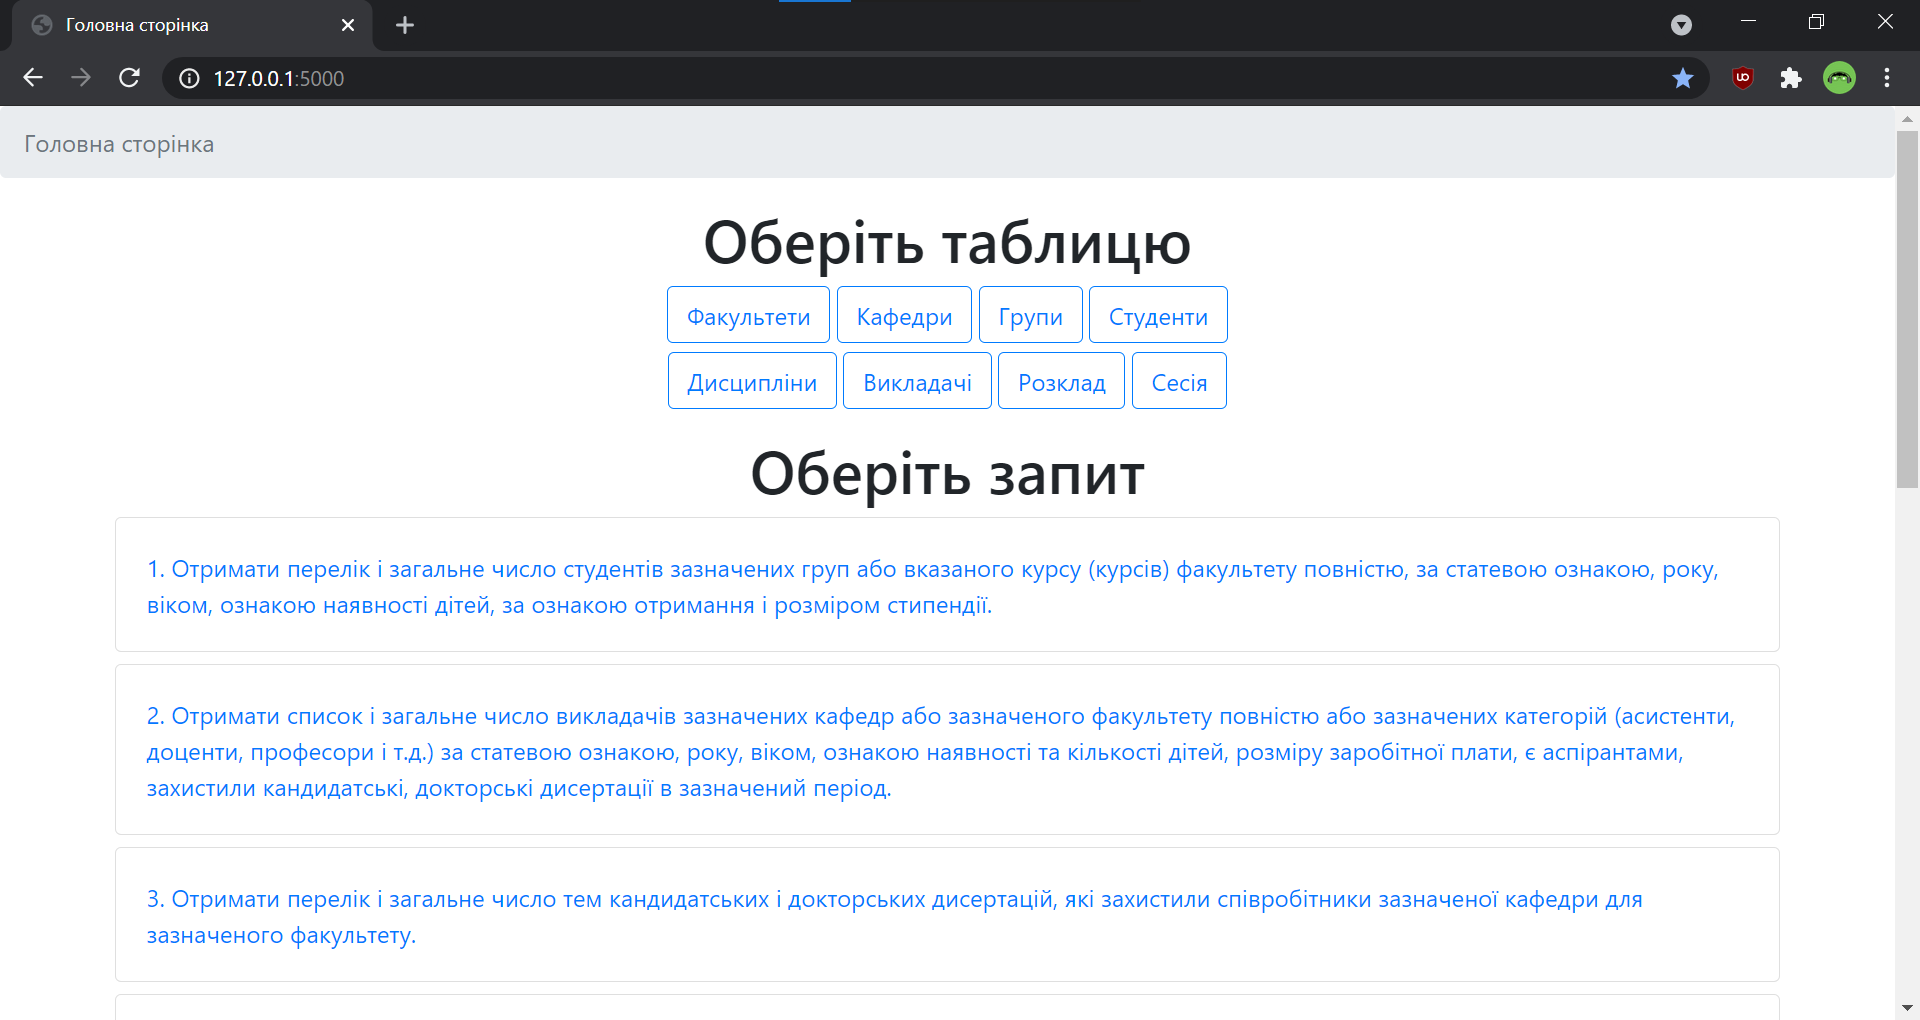
\includegraphics[scale=0.38]{pics/web_main.png}
    \caption{Головна сторінка веб-інтерфейсу}
\end{figure}

\begin{figure}[H]
    \centering
    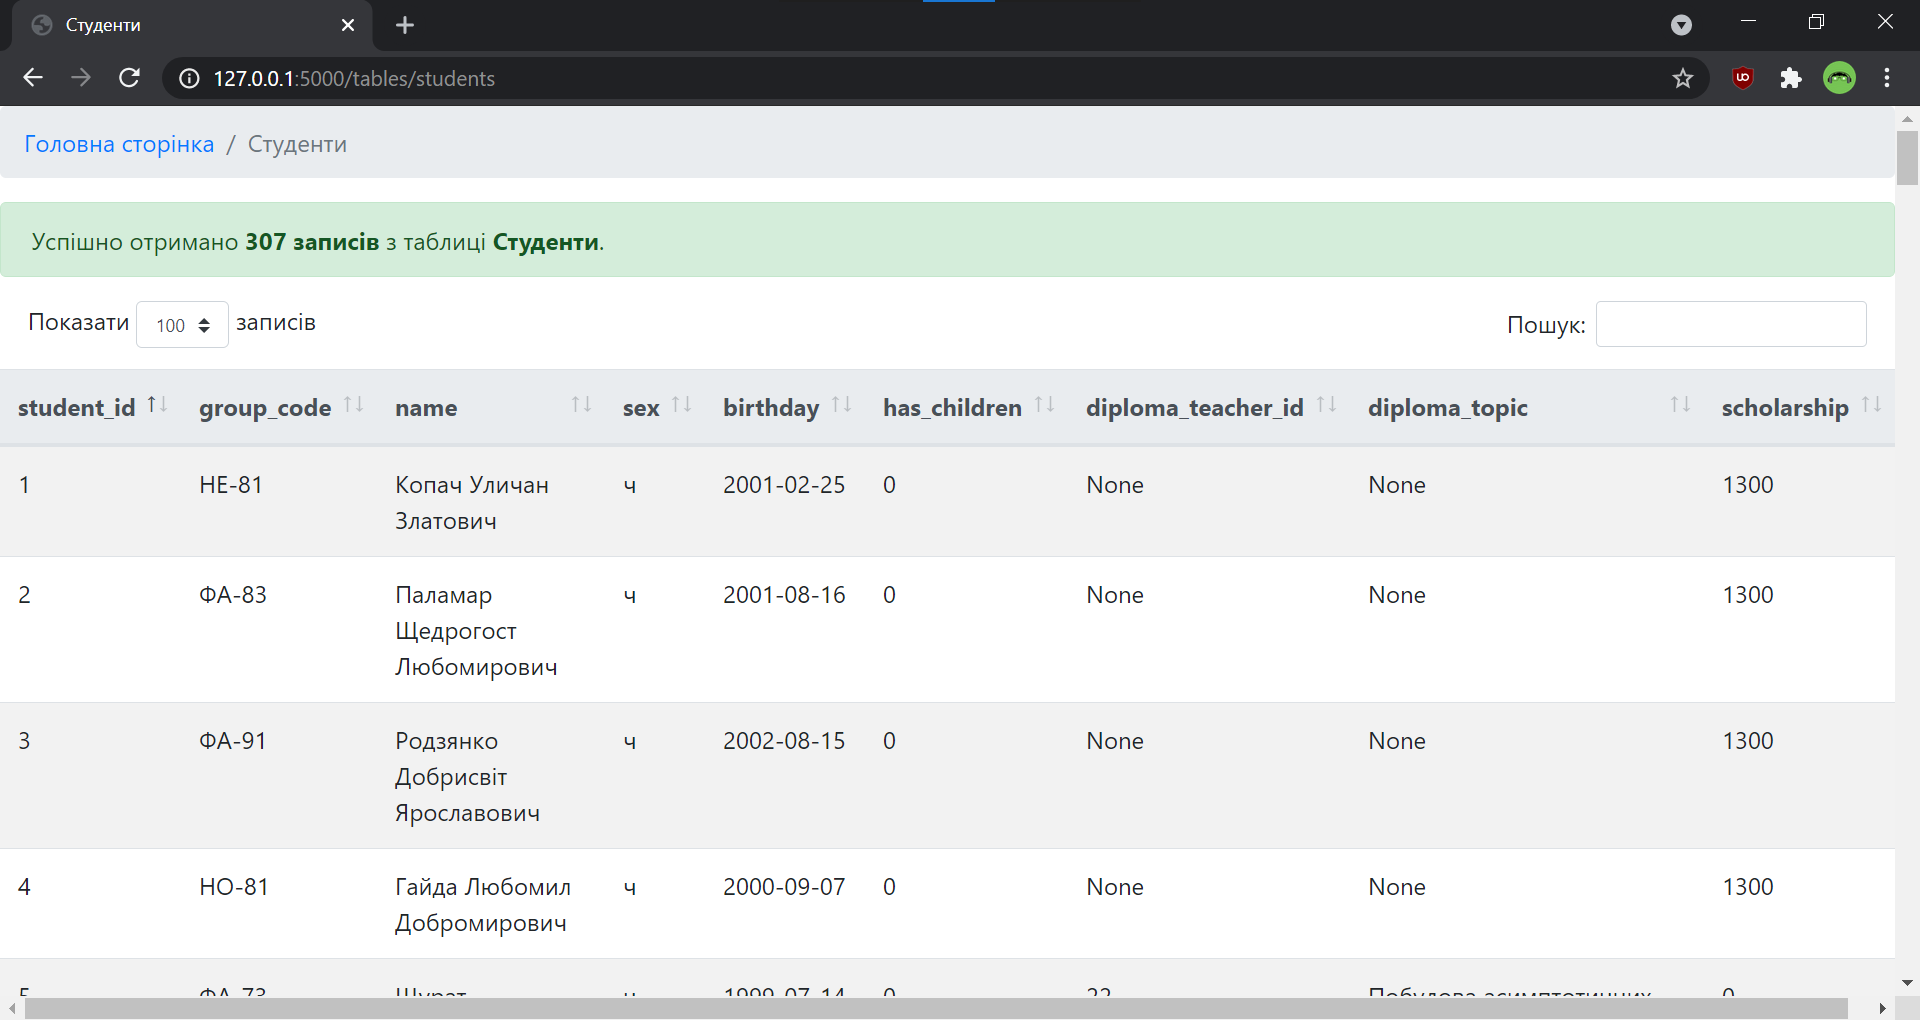
\includegraphics[scale=0.38]{pics/web_table.png}
    \caption{Перегляд таблиці <<Студенти>>}
\end{figure}

\begin{figure}[H]
    \centering
    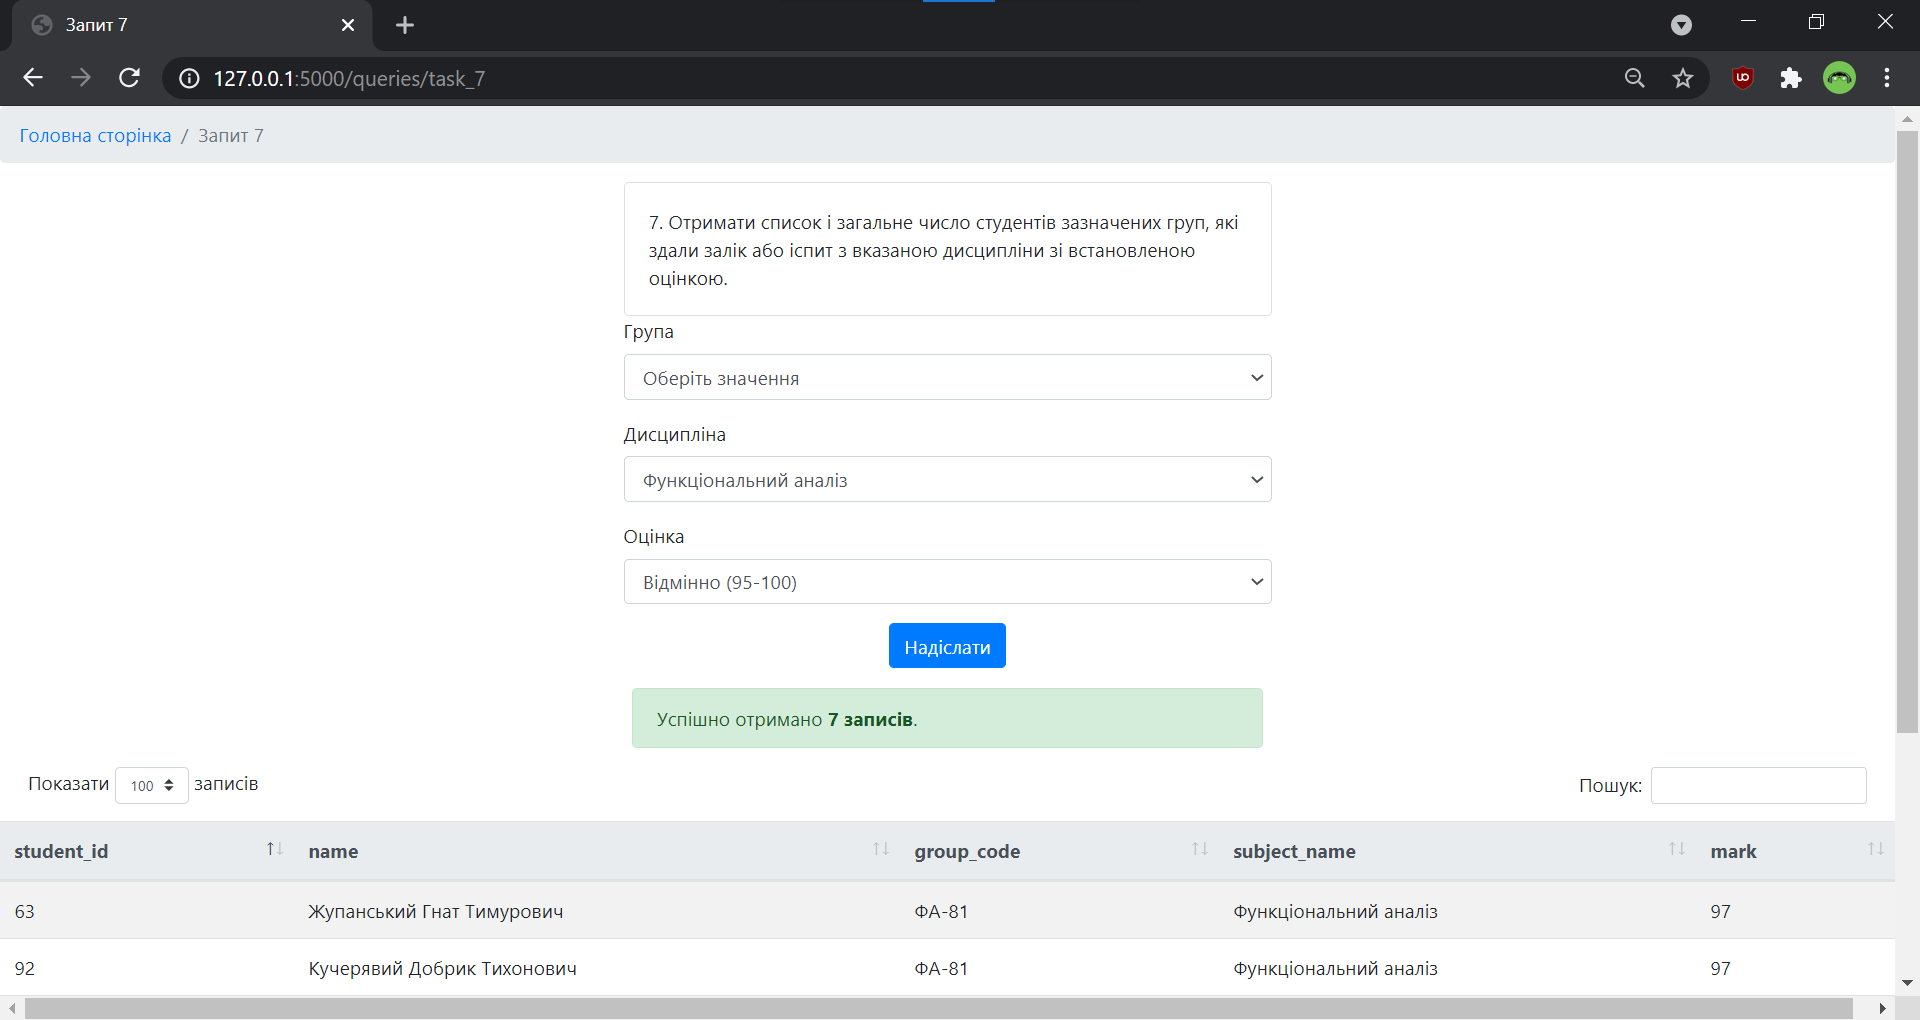
\includegraphics[scale=0.38]{pics/web_query.png}
    \caption{Форма для запиту та результат виконання}
\end{figure}

\section{Реалізація механізмів БД}
Реалізовано 13 процедур, що відповідають поставленим вимогам до запитів.
SQL-код цих процедур наведено в додатку 3, ст. \pageref{queries}. Виклик усіх процедур
відбувається через веб-інтерфейс і користувачу не потрібно писати назву чи параметри процедури вручну.